\chapter{Jeffreys Priors and Bayesian Intervals}
\label{ch:jeffreys}

\begin{chaptergoals}
\begin{itemize}[nosep]
\item What a prior for `knowing nothing' can be, and why the flat prior gives a different answer on each scale a parameter can be written on: the proportion $p$ against its log-odds, a rate against a mean wait.
\item Improper priors, whose densities have an infinite integral: when they still give a proper posterior, when they give none, and why they cannot be the prior for the parameter that a point null fixes.
\item Jeffreys' prior, built from the Fisher information so that changing the parameterization changes nothing: $\Betad(\frac12, \frac12)$ for the kiss data, $1/\lambda$ for the subway rate, $1/\sigma$ for a scale. Why it puts equal mass on what the data can tell apart.
\item Bayesian confidence regions, equal-tailed and highest-density, and what their $95\%$ means. When they coincide with the intervals of \cref{ch:confidence-intervals,ch:t-test} exactly (the subway's exact interval, the $t$-interval) and when only for large $n$ (Bernstein--von Mises).
\end{itemize}
\Cref{ch:bayes-intro} turned a prior and the likelihood into a posterior. This chapter asks which prior to use when there is nothing to put in one, and what the posterior's intervals mean.
\end{chaptergoals}

\section{A prior for knowing nothing}
\label{sec:jeff-flat}

Every posterior in \cref{ch:bayes-intro} started from a prior somebody chose: a timetable's promise for the subway, a regional average for the wind turbine, a skeptic's $90\%$ belief for the kiss data.
Often there is nothing of the sort to write down, or the point of the analysis is to report what the data say on their own.
The oldest answer is to give every value of the parameter the same density.
Bayes (1763) did this for a proportion, and Laplace made it a rule, later called the principle of insufficient reason: with no reason to prefer one value, prefer none.
For the kiss data the flat prior gives the posterior $\Betad(81, 45)$ of \cref{thm:beta-bernoulli}, with mean $0.643$ and middle $95\%$ from $0.558$ to $0.724$.

The trouble is that `the same density for every value' depends on how the values are written.
The kiss proportion $p$ can just as well be described by its log-odds, $\psi = \log(p/(1-p))$, the scale on which logistic regression works (\cref{ch:glm-links}), and someone who knows nothing about $p$ knows nothing about $\psi$ either.
But a flat density for $p$ is not flat for $\psi$.
To find the density of $\psi$, write its CDF and differentiate \toolkit{sec:math-density}: for a strictly increasing smooth map $\psi = g(p)$, $\Pr(\psi \leq u) = \Pr(p \leq g^{-1}(u))$, and the derivative in $u$ is the density of $p$ at $g^{-1}(u)$ times the derivative of $g^{-1}$.
In general, for a smooth one-to-one map $\varphi = g(\theta)$,
\begin{equation}
\label{eq:jeff-change}
\pi_\varphi(\varphi) = \pi_\theta(\theta)\,\abs*{\frac{\mathrm{d}\theta}{\mathrm{d}\varphi}}, \qquad \theta = g^{-1}(\varphi),
\end{equation}
where the absolute value covers decreasing maps.
For the log-odds, $p = e^\psi/(1 + e^\psi)$ and $\mathrm{d}p/\mathrm{d}\psi = p(1-p)$, so the flat prior on $p$ becomes the density $p(1-p) = e^\psi/(1 + e^\psi)^2$ on $\psi$: the logistic density, peaked at $\psi = 0$, which is $p = \frac12$.
It is far from ignorant about $\psi$: it puts probability $0.90$ on $\abs{\psi} \leq 2.94$, which is the event $0.05 \leq p \leq 0.95$.
Run the other way, a flat prior on $\psi$ becomes the density $1/(p(1-p))$ on $p$, which piles up at $0$ and at $1$.

\Cref{fig:jeffscales} draws this, together with the prior this chapter ends up recommending.
On the left, on the scale of $p$, the flat prior is the blue line.
On the right, on the scale of $\psi$, the same prior is the blue bell, while the flat rule applied to $\psi$ directly gives the gray line: two people who both claim to know nothing about the kiss data, one thinking in $p$ and one in $\psi$, start from different priors and end with different posteriors.
The orange curves are Jeffreys' prior of \cref{sec:jeff-prior}, a U on the left and a wider bell on the right.
The orange dots on the right were computed on $\psi$ directly, by Jeffreys' rule, and they land on the orange curve: that rule gives one answer on both scales.

\begin{figure}[htbp]
\centering
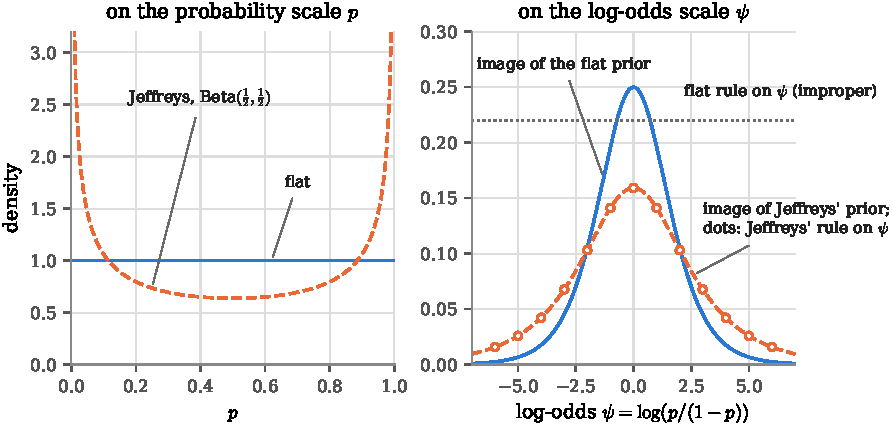
\includegraphics[width=\textwidth]{fig_jeffreys_scales}
\caption{Two priors for the kiss proportion. Left, on $p$: flat (blue) and Jeffreys' $\Betad(\frac12, \frac12)$ (orange, dashed). Right, on the log-odds $\psi$: their images (same colors), the flat rule on $\psi$ (gray dotted, height arbitrary) and Jeffreys' rule on $\psi$ (orange dots).}
\label{fig:jeffscales}
\end{figure}

The subway gives a second example.
Its rate $\lambda$, in trains per minute, and its mean wait $\beta = 1/\lambda$, in minutes per train, are two descriptions of one parameter.
A flat prior on $\lambda$ is the density $1$ on $(0, \infty)$; a flat prior on $\beta$ becomes, by \cref{eq:jeff-change} with $\abs{\mathrm{d}\beta/\mathrm{d}\lambda} = 1/\lambda^2$, the density $1/\lambda^2$ on $\lambda$.
The $64$ waits total $398.7$ minutes, so the likelihood is $\lambda^{64}e^{-398.7\lambda}$ (\cref{ch:likelihood}), and the two posteriors are $\Gammad(65, 398.7)$ and $\Gammad(63, 398.7)$, with means $0.163$ and $0.158$ trains per minute and middle $95\%$ intervals $[0.126, 0.205]$ and $[0.121, 0.199]$.
Neither prior has a finite integral, which \cref{sec:jeff-improper} takes up, yet both posteriors are ordinary Gamma distributions.
At $n = 64$ the two posterior means differ by a quarter of a posterior standard deviation ($0.005$ against $0.020$), a difference produced by nothing but the choice between `rate' and `wait'.

\begin{pitfall}[`uninformative' is not a property of a prior alone]
A prior that is flat for $p$ is informative about $\psi$, about $p^2$ and about every other nonlinear function of $p$, and no density is flat on every scale at once.
`I used a flat prior' says nothing until it says flat \textit{in what}.
\Cref{ch:bayes-intro} met the same problem from the other side: the posterior mode moved from $0.645$ to $0.643$ when the kiss data were described by their log-odds (\cref{ex:bayes-map}) because a mode is where a density peaks, and densities change under a change of variables.
\end{pitfall}

\section{Improper priors}
\label{sec:jeff-improper}

The flat prior on the subway rate gives every $\lambda > 0$ the same density, and $\int_0^\infty 1\,\mathrm{d}\lambda = \infty$, so no rescaling makes it a probability distribution and \cref{def:posterior}, which asks for one, does not cover it.
Yet the posterior it produced, $\Gammad(65, 398.7)$, is an ordinary distribution.
Bayes' formula uses the prior only through the product $L_n\pi$ and its integral, and those can be finite when the integral of $\pi$ is not.

\begin{definition}[Improper prior]
\label{def:improper-prior}
An \textbf{improper prior} on $\Theta$ is a nonnegative function $\pi$ on $\Theta$ with $\int_\Theta \pi(\theta)\,\mathrm{d}\theta = \infty$. For data $\mathbf{x}$ with
\[
0 < m(\mathbf{x}) = \int_\Theta L_n(\mathbf{x}; t)\,\pi(t)\,\mathrm{d}t < \infty,
\]
its \textbf{posterior} is $\pi(\theta \mid \mathbf{x}) = L_n(\mathbf{x}; \theta)\,\pi(\theta)/m(\mathbf{x})$, a probability density on $\Theta$. A prior with a finite integral, rescaled to integrate to $1$, is called \textbf{proper}.
\end{definition}

\begin{inwords}
\textbf{In words.} An improper prior is a weighting of the parameter values whose total weight is infinite, so it is not a distribution. It is used only through Bayes' formula: when likelihood times prior has a finite integral, the posterior is a genuine distribution, and when it does not, there is no posterior. Multiplying an improper prior by a constant changes nothing, since the constant cancels.
\par\smallskip
\textbf{For the kiss data.} The flat prior on the log-odds, $\pi(p) = 1/(p(1-p))$ on $(0, 1)$, is improper: its integral diverges at both ends. Times the likelihood $p^{80}(1-p)^{44}$ it gives $p^{79}(1-p)^{43}$, which has a finite integral, so the posterior is $\Betad(80, 44)$, with mean $80/124 = 0.645$, the sample proportion.
\end{inwords}

This prior is known as Haldane's prior, after J. B. S. Haldane (\textit{Proceedings of the Cambridge Philosophical Society}, 1932).
Where improper priors come from is easiest to see for a Gaussian mean with $\sigma$ known.
There \cref{prop:normal-normal} turned the prior $\Gauss(\mu_0, \sigma_0^2)$ into a posterior with precision $1/\sigma_0^2 + n/\sigma^2$, whose mean is the precision-weighted average of $\mu_0$ and $\bar{x}$.

\begin{intuition}[an improper prior is the limit of wider and wider proper ones]
Let the prior's standard deviation $\sigma_0$ grow.
The prior flattens toward the constant $0$, which is no density at all, but the posterior settles down: its precision tends to $n/\sigma^2$ and its mean to $\bar{x}$, so the posterior tends to $\Gauss(\bar{x}, \sigma^2/n)$.
That limit is what the improper flat prior $\pi(\mu) = 1$ gives in one step, since the likelihood is $\exp(-n(\mu - \bar{x})^2/(2\sigma^2))$ times a factor free of $\mu$, already a Gaussian shape in $\mu$.
For the wind turbine with $\sigma = 4.7$ treated as known, the prior centered at $11$ with $\sigma_0 = 2$ gave posterior mean $13.26$; with $\sigma_0 = 10$ the mean is $14.24$, and in the limit it is $\bar{x} = 14.3$, with standard deviation $4.7/\sqrt{12} = 1.36$.
An improper prior is shorthand for `a prior so wide that its exact width does not matter'.
\end{intuition}

The condition $m(\mathbf{x}) < \infty$ in \cref{def:improper-prior} is the price of that shorthand, and it can fail.

\begin{pitfall}[an improper prior can give no posterior]
Under Haldane's prior, suppose all $n$ couples had turned right.
Then $L_n\pi = p^{n-1}(1-p)^{-1}$, whose integral diverges at $p = 1$, and there is no posterior at all.
The formula still produces a function, and normalizing it numerically on a grid even produces a picture, but the picture depends on where the grid stops.
With a proper prior and discrete data this cannot happen, since then $m(\mathbf{x}) \leq 1$.
The results of \cref{ch:bayes-intro} that assume a prior distribution, \cref{thm:bvm} among them, do not apply as stated to an improper prior; for the improper priors of this chapter the Gaussian limit can be checked directly, since their posteriors are Gamma, Beta, Gaussian and $t$ distributions.
\end{pitfall}

Estimation and intervals tolerate improper priors because the arbitrary constant in front of the prior cancels between numerator and denominator.
One calculation of \cref{ch:bayes-intro} has no denominator to cancel it.

\begin{pitfall}[no improper prior for the parameter a point null fixes]
\Cref{sec:bayes-hypotheses} compared $H_0: p = \frac12$ with $H_1: p \neq \frac12$ through the Bayes factor $B_{01} = m_0/m_1$, where $m_1$ averages the likelihood over the prior on the alternative.
If that prior is improper, it is defined only up to a constant $c$, and $c$ multiplies $m_1$ but not $m_0$, which is computed at the single value $p = \frac12$: the Bayes factor, and $\Pr(H_0 \mid \mathbf{x})$ with it, can be made anything.
With Haldane's prior on the alternative, for instance, $B_{01}$ is $0.011$ for $c = 1$ and $0.000011$ for $c = 1{,}000$ (\cref{ex:jeff-bayes-factor}).
For testing, Jeffreys himself used proper priors for the parameter under test, such as a Cauchy prior for a Gaussian mean, and kept the improper $1/\sigma$ only for the $\sigma$ that both hypotheses share, whose constant cancels between $m_0$ and $m_1$.
\end{pitfall}

\section{Jeffreys' prior}
\label{sec:jeff-prior}

The flat prior failed because `constant density' is a rule that produces a different prior on each scale it is applied to.
Harold Jeffreys (\textit{Proceedings of the Royal Society A}, 1946) asked for a rule that does not: apply it on the scale of $\theta$ and carry the result to $\varphi = g(\theta)$ by \cref{eq:jeff-change}, or apply it on the scale of $\varphi$ directly, and get the same prior either way.
A fixed formula in $\theta$ cannot do this, since it ignores the factor $\abs{\mathrm{d}\theta/\mathrm{d}\varphi}$ that every change of variables puts on a density.
The rule has to be built from something attached to the model that changes with the parameterization in step with densities, and the Fisher information is such a thing.

\recall{The Fisher information of one observation (\cref{def:fisher}, \cref{thm:fisher-curvature}): for a model satisfying the regularity conditions of \cref{sec:mle-regularity}, $I(\theta) = \E_\theta[\ell'(\theta)^2] = -\E_\theta[\ell''(\theta)]$, where $\ell$ is the log-likelihood of one observation. A large $I(\theta)$ means one observation pins $\theta$ down well: the maximum likelihood estimator has asymptotic variance $1/I(\theta)$, so its standard error is about $1/\sqrt{nI(\theta)}$ (\cref{thm:mle-normal}).}

\begin{lemma}[Fisher information under a change of parameter]
\label{lem:fisher-reparam}
Let $\varphi = g(\theta)$ with $g$ smooth and one-to-one and $g' \neq 0$, and write $I_\theta$ and $I_\varphi$ for the Fisher information of one observation in the two parameterizations. Then
\[
I_\varphi(\varphi) = I_\theta(\theta)\Big(\frac{\mathrm{d}\theta}{\mathrm{d}\varphi}\Big)^2, \qquad \theta = g^{-1}(\varphi).
\]
\end{lemma}

\optionalproof{By the chain rule the score in $\varphi$ is the score in $\theta$ times the number $\mathrm{d}\theta/\mathrm{d}\varphi$, and a constant factor comes out of a variance squared.}
\begin{proof}
The model is the same, only the labels of its members change: the observation's density at the member labeled $\varphi$ is $p_{g^{-1}(\varphi)}(x)$. So the log-likelihood in $\varphi$ is $\tilde{\ell}(\varphi) = \ell(g^{-1}(\varphi))$, and by the chain rule $\tilde{\ell}'(\varphi) = \ell'(\theta)\,\mathrm{d}\theta/\mathrm{d}\varphi$ with $\theta = g^{-1}(\varphi)$. The factor $\mathrm{d}\theta/\mathrm{d}\varphi$ is a number, not a random variable, so $\var(\tilde{\ell}'(\varphi)) = (\mathrm{d}\theta/\mathrm{d}\varphi)^2\var(\ell'(\theta))$, which is the claim.
\end{proof}

\Cref{ex:mle-reparam} checked the lemma for the subway: $I = 1/\lambda^2$ for the rate and $1/\beta^2$ for the mean wait.
Which function of the information should the prior be?
Try a power, $\pi(\theta) \propto I_\theta(\theta)^a$.
Applied on the scale of $\theta$ and carried to $\varphi$ by \cref{eq:jeff-change}, it gives $I_\theta(\theta)^a\abs{\mathrm{d}\theta/\mathrm{d}\varphi}$.
Applied on the scale of $\varphi$ directly, it gives, by \cref{lem:fisher-reparam}, $I_\varphi(\varphi)^a = I_\theta(\theta)^a\abs{\mathrm{d}\theta/\mathrm{d}\varphi}^{2a}$.
The two are proportional for every change of variables only if $\abs{\mathrm{d}\theta/\mathrm{d}\varphi}^{2a - 1}$ is constant whatever $g$ is, and that forces $2a = 1$.

\begin{definition}[Jeffreys' prior]
\label{def:jeffreys}
For a one-parameter model with Fisher information $I(\theta)$, \textbf{Jeffreys' prior} is
\[
\pi_J(\theta) \propto \sqrt{I(\theta)},
\]
proper or improper according to whether $\int_\Theta \sqrt{I(\theta)}\,\mathrm{d}\theta$ is finite. For $\theta \in \real^d$ with Fisher information matrix $I(\theta)$, it is $\pi_J(\theta) \propto \sqrt{\det I(\theta)}$.
\end{definition}

\begin{inwords}
\textbf{In words.} Take the information one observation carries about $\theta$, take its square root, and use that as the prior density, up to a constant. The prior depends on the model, through $I$, and on nothing else: not on the data, not on anyone's beliefs. Using the information of all $n$ observations, $nI(\theta)$, gives the same prior, since the factor $\sqrt{n}$ is a constant.
\par\smallskip
\textbf{For the kiss data.} $I(p) = 1/(p(1-p))$ (\cref{sec:mle-fisher-examples}), so $\pi_J(p) \propto p^{-1/2}(1-p)^{-1/2}$: the $\Betad(\frac12, \frac12)$ density, which is proper, with constant $1/\pi$. The posterior is $\Betad(80.5, 44.5)$, with mean $80.5/125 = 0.644$ and middle $95\%$ from $0.558$ to $0.725$, where the flat prior gave $0.643$ and $[0.558, 0.724]$.
\end{inwords}

\begin{theorem}[Jeffreys' prior does not depend on the parameterization]
\label{thm:jeffreys-invariant}
Let $\varphi = g(\theta)$ with $g$ smooth and one-to-one and $g' \neq 0$. If $\theta$ has the prior $\pi_J^\theta \propto \sqrt{I_\theta}$, then the prior that \cref{eq:jeff-change} gives $\varphi$ is proportional to $\sqrt{I_\varphi(\varphi)}$, which is Jeffreys' prior for the model written in terms of $\varphi$. The same holds in $\real^d$, with $\sqrt{\det I}$ and the determinant of the matrix of partial derivatives.
\end{theorem}

\coreproof{The factor that a change of variables puts on a density is exactly the factor by which the square root of the information changes.}
\begin{proof}
By \cref{eq:jeff-change} and \cref{lem:fisher-reparam},
\[
\pi_J^\theta(\theta)\abs*{\frac{\mathrm{d}\theta}{\mathrm{d}\varphi}} \propto \sqrt{I_\theta(\theta)}\,\abs*{\frac{\mathrm{d}\theta}{\mathrm{d}\varphi}} = \sqrt{I_\theta(\theta)\Big(\frac{\mathrm{d}\theta}{\mathrm{d}\varphi}\Big)^2} = \sqrt{I_\varphi(\varphi)}.
\]
In $\real^d$, write $J$ for the $d \times d$ matrix of partial derivatives $\partial\theta_i/\partial\varphi_j$. The chain rule makes the score in $\varphi$ equal to $J^\top$ times the score in $\theta$, so $I_\varphi = J^\top I_\theta J$ and $\det I_\varphi = (\det J)^2\det I_\theta$. The density of $\varphi$ is the density of $\theta$ times $\abs{\det J}$ (the substitution rule of multivariable calculus, whose linear case is the change of variables formula of \toolkit{sec:math-gaussvec}: near each point the map from $\varphi$ to $\theta$ is, up to a shift and a negligible error, the linear map $J$, which multiplies small volumes by $\abs{\det J}$), and $\sqrt{\det I_\theta}\,\abs{\det J} = \sqrt{\det I_\varphi}$.
\end{proof}

\begin{worked}[the kiss data on the log-odds scale]
On $\psi = \log(p/(1-p))$, $\mathrm{d}p/\mathrm{d}\psi = p(1-p)$, so \cref{lem:fisher-reparam} gives $I_\psi(\psi) = \frac{1}{p(1-p)}\,p^2(1-p)^2 = p(1-p)$, and Jeffreys' rule applied on $\psi$ gives $\pi_J(\psi) \propto \sqrt{p(1-p)}$, with $p = e^\psi/(1 + e^\psi)$.
Carrying $\Betad(\frac12, \frac12)$ over by \cref{eq:jeff-change} instead gives $\frac{1}{\pi\sqrt{p(1-p)}}\,p(1-p) = \sqrt{p(1-p)}/\pi$: the same function, now with its constant.
In terms of $\psi$ it is $1/(2\pi\cosh(\psi/2))$, the orange curve on the right of \cref{fig:jeffscales}, and the orange dots there are $\sqrt{I_\psi}/\pi$ at whole numbers $\psi$.
The flat rule has no such property: applied on $p$ and carried over it gives the logistic density $p(1-p)$, and applied on $\psi$ it gives a constant.
\end{worked}

Why the square root of the information, beyond the algebra?
The information measures how finely the data can tell neighboring values of $\theta$ apart, and Jeffreys' prior turns out to give every distinguishable stretch of the parameter the same share.

\begin{intuition}[equal mass for what the data can tell apart]
Near a value $\theta$, the $95\%$ interval of \cref{ch:confidence-intervals} has half-width about $1.96/\sqrt{nI(\theta)}$: values closer than that are hard to tell apart with $n$ observations, and values much farther apart are easy.
Where $I(\theta)$ is large these intervals are narrow and many of them fit into a unit of $\theta$; where it is small they are wide.
Jeffreys' prior gives each of them the same mass: its density $\sqrt{I(\theta)}$ times the width $3.92/\sqrt{nI(\theta)}$ is $3.92/\sqrt{n}$, whatever $\theta$ is.
For the kiss model the binomial pins $p$ down tightly near $0$ and $1$, where $p(1-p)$ is small, and loosely near $\frac12$, so the U of $\Betad(\frac12, \frac12)$ is the shape that gives every distinguishable interval the same share.
\Cref{fig:jeffequalmass} shows five such intervals at $n = 124$: narrow under the tall ends of the U, wide under its low middle, and each with Jeffreys mass between $0.113$ and $0.116$ (the approximation $3.92/(\pi\sqrt{124})$, with the constant $1/\pi$, gives $0.112$).
\end{intuition}

\begin{figure}[htbp]
\centering
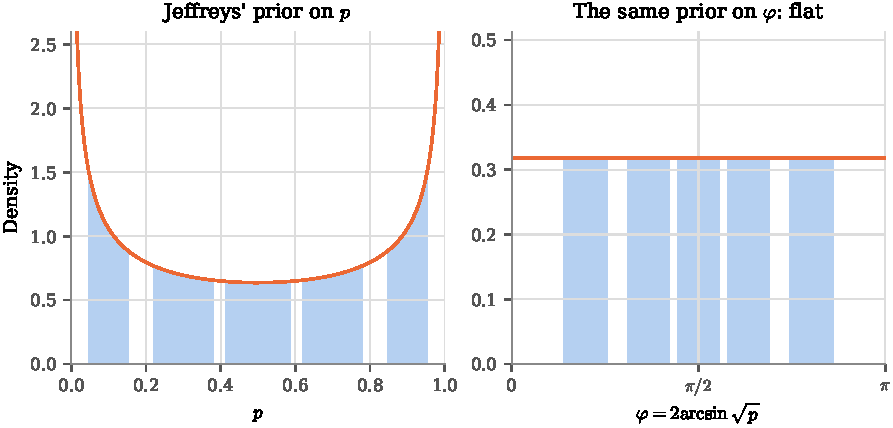
\includegraphics[width=\textwidth]{fig_jeffreys_equal_mass}
\caption{Jeffreys' prior for the kiss proportion (orange) with five bands $p_0 \pm 1.96\sqrt{p_0(1-p_0)/124}$, for $p_0 = 0.1, 0.3, 0.5, 0.7, 0.9$ (blue). Left: on $p$. Right: on $\varphi = 2\arcsin\sqrt{p}$, where the prior is flat.}
\label{fig:jeffequalmass}
\end{figure}

On the right of \cref{fig:jeffequalmass} the same bands are drawn on the scale $\varphi = 2\arcsin\sqrt{p}$, where they all have nearly the same width and the prior is flat.
That is not a coincidence: every one-parameter model has a scale on which its Jeffreys prior is flat.

\begin{proposition}[Jeffreys' prior is flat where the information is constant]
\label{prop:jeffreys-stabilizing}
In a one-parameter model satisfying the regularity conditions of \cref{sec:mle-regularity}, with $\Theta$ an interval and $I(\theta)$ continuous and positive on it, let $\varphi(\theta) = \int_{\theta_0}^\theta \sqrt{I(t)}\,\mathrm{d}t$ for a fixed $\theta_0 \in \Theta$. Then $I_\varphi \equiv 1$, Jeffreys' prior is flat in $\varphi$, and the maximum likelihood estimator satisfies $\sqrt{n}\big(\varphi(\hat{\theta}_n) - \varphi(\theta)\big) \convd \Gauss(0, 1)$ under $\Pr_\theta$ for every $\theta$ in the interior of $\Theta$: $\varphi$ is a variance-stabilizing transformation.
\end{proposition}

\recall{The delta method (\cref{thm:delta}): if $\sqrt{n}(Z_n - \theta) \convd \Gauss(0, \tau^2)$ and $g$ is continuously differentiable at $\theta$, then $\sqrt{n}\big(g(Z_n) - g(\theta)\big) \convd \Gauss\big(0, g'(\theta)^2\tau^2\big)$.}

\optionalproof{\Cref{lem:fisher-reparam} with $\mathrm{d}\varphi/\mathrm{d}\theta = \sqrt{I(\theta)}$, then the delta method.}
\begin{proof}
By the fundamental theorem of calculus, $\mathrm{d}\varphi/\mathrm{d}\theta = \sqrt{I(\theta)} > 0$, so $\varphi$ is strictly increasing, and \cref{lem:fisher-reparam} gives $I_\varphi = I_\theta(\mathrm{d}\theta/\mathrm{d}\varphi)^2 = I_\theta/I_\theta = 1$. Jeffreys' prior in $\varphi$ is then proportional to $\sqrt{1}$, a constant. By \cref{thm:mle-normal}, $\sqrt{n}(\hat{\theta}_n - \theta) \convd \Gauss(0, 1/I(\theta))$, and the delta method with $g = \varphi$, whose derivative $\sqrt{I}$ is continuous, gives the asymptotic variance $I(\theta) \cdot 1/I(\theta) = 1$.
\end{proof}

For the Bernoulli, $\int \mathrm{d}p/\sqrt{p(1-p)} = 2\arcsin\sqrt{p}$, which is why $\Betad(\frac12, \frac12)$ is also called the arcsine distribution.
For the Poisson, $I(\lambda) = 1/\lambda$ and $\varphi = 2\sqrt{\lambda}$.
For the exponential rate, $I(\lambda) = 1/\lambda^2$ and $\varphi = \log\lambda$: Jeffreys' prior $1/\lambda$ is flat in $\log\lambda$, and since $\log\beta = -\log\lambda$ it is flat in the log of the mean wait too.
So for the subway, where the flat prior on the rate and the flat prior on the wait disagreed (\cref{sec:jeff-flat}), Jeffreys' rule gives one answer: the prior $1/\lambda$ for the rate is the prior $1/\beta$ for the wait, and the posterior is $\Gammad(64, 398.7)$, between the two flat answers, with posterior mean $64/398.7 = 0.1605$, the maximum likelihood estimate.

\begin{bridge}[the arcsine and square-root transformations]
Applied courses in experimental design traditionally transform proportions by $\arcsin\sqrt{\hat{p}}$ and counts by $\sqrt{x}$ before comparing groups, so that every group has about the same variance whatever its mean.
These are the transformations of \cref{prop:jeffreys-stabilizing} for the Bernoulli and Poisson models, up to the factor $2$.
On those scales the Fisher information is constant, the standard error of the transformed estimate is $1/\sqrt{n}$ whatever the parameter, and Jeffreys' prior is flat.
For the kiss data, $2\arcsin\sqrt{0.645} = 1.865$ with standard error $1/\sqrt{124} = 0.090$, and the interval $1.865 \pm 1.96 \times 0.090$, mapped back to $p$, is $[0.559, 0.727]$, close to the Jeffreys posterior interval $[0.558, 0.725]$.
\end{bridge}

The table collects Jeffreys' prior for the book's one-parameter families, with the posterior after $n$ observations whose sum is $S$.
Only the first prior is proper, and each posterior is proper: for the Bernoulli always, for the Poisson, the exponential and the Gaussian mean once $n \geq 1$, and for the Gaussian scale once $n \geq 1$ and not every $x_i$ equals $\mu$.

\begin{center}
\small
\begin{tabular}{@{}llll@{}}
\toprule
model & $I$ & Jeffreys' prior & posterior \\
\midrule
$\Bern(p)$ & $1/(p(1-p))$ & $\Betad(\frac12, \frac12)$ & $\Betad(S + \frac12, n - S + \frac12)$ \\[2pt]
$\Pois(\lambda)$ & $1/\lambda$ & $\lambda^{-1/2}$, improper & $\Gammad(S + \frac12, n)$ \\[2pt]
$\Expo(\lambda)$ & $1/\lambda^2$ & $1/\lambda$, improper & $\Gammad(n, S)$ \\[2pt]
$\Gauss(\mu, \sigma^2)$, $\sigma$ known & $1/\sigma^2$ & $1$, improper & $\Gauss(\bar{x}, \sigma^2/n)$ \\[2pt]
$\Gauss(\mu, \sigma^2)$, $\mu$ known, in $\sigma$ & $2/\sigma^2$ & $1/\sigma$, improper & $\sum_i(x_i - \mu)^2/\sigma^2 \sim \chi^2_n$ \\
\bottomrule
\end{tabular}
\end{center}

\section{Several parameters: a Gaussian with unknown variance}
\label{sec:jeff-several}

\Cref{ch:bayes-intro} needed a prior for the wind turbine's $\sigma$ when it was unknown, used a density proportional to $1/\sigma$, independent of $\mu$, and promised this chapter would explain it.
The last row of the table is the explanation: $1/\sigma$ is Jeffreys' prior for $\sigma$ when $\mu$ is known, flat in $\log\sigma$.
With both parameters unknown, \cref{def:jeffreys} asks for the information matrix.
\Cref{sec:mle-fisher-examples} computed it for $(\mu, \sigma^2)$, and the matrix rule $I_\varphi = J^\top I_\theta J$ from the proof of \cref{thm:jeffreys-invariant}, with $J$ diagonal and $\mathrm{d}\sigma^2/\mathrm{d}\sigma = 2\sigma$, turns its entry $1/(2\sigma^4)$ into $(2\sigma)^2/(2\sigma^4) = 2/\sigma^2$:
\[
I(\mu, \sigma) = \begin{pmatrix} 1/\sigma^2 & 0 \\ 0 & 2/\sigma^2 \end{pmatrix}, \qquad \sqrt{\det I(\mu, \sigma)} = \frac{\sqrt{2}}{\sigma^2}.
\]
So Jeffreys' rule applied to $(\mu, \sigma)$ together gives the prior $1/\sigma^2$, not $1/\sigma$.
Jeffreys himself noticed the difference and recommended treating a location and a scale separately, each with its own one-parameter rule: flat in $\mu$, times $1/\sigma$.
The next result shows what the extra factor of $1/\sigma$ does.

\begin{proposition}[The posterior of a Gaussian mean with unknown variance]
\label{prop:jeff-t-posterior}
Given $(\mu, \sigma)$, let $\Xton$ be i.i.d.\ $\Gauss(\mu, \sigma^2)$, with $n \geq 2$, and let $\bar{x}$ and $s > 0$ be the observed sample mean and sample standard deviation. Take the improper prior $\pi(\mu, \sigma) = \sigma^{-k}$ on $\real \times (0, \infty)$, with $k = 1$ or $k = 2$. Then the posterior is proper, and the posterior distribution of $\mu$, with $\bar{x}$ and $s$ fixed, is given by
\[
\frac{\mu - \bar{x}}{s/\sqrt{n}} \sim t_{n-1} \quad (k = 1), \qquad \frac{\mu - \bar{x}}{s\sqrt{(n-1)/n}\big/\sqrt{n}} \sim t_n \quad (k = 2).
\]
\end{proposition}

\coreproof{Write the likelihood with $\sum_i(x_i - \mu)^2 = (n-1)s^2 + n(\bar{x} - \mu)^2$, integrate $\sigma$ out with a Gamma integral, and recognize Student's $t$ density in what is left.}
\begin{proof}
Adding and subtracting $\bar{x}$ inside the square, the cross term vanishes, and $A(\mu) = \sum_i(x_i - \mu)^2 = (n-1)s^2 + n(\bar{x} - \mu)^2$. The likelihood is $(2\pi)^{-n/2}\sigma^{-n}\exp(-A(\mu)/(2\sigma^2))$, so the posterior is proportional to $\sigma^{-(n+k)}\exp(-A(\mu)/(2\sigma^2))$. For fixed $\mu$, substitute $u = A(\mu)/(2\sigma^2)$, so that $\sigma = (A(\mu)/(2u))^{1/2}$ and $\mathrm{d}\sigma = -\frac12(A(\mu)/2)^{1/2}u^{-3/2}\,\mathrm{d}u$:
\begin{align*}
\int_0^\infty \sigma^{-(n+k)}e^{-A(\mu)/(2\sigma^2)}\,\mathrm{d}\sigma &= \frac12\Big(\frac{A(\mu)}{2}\Big)^{-(n+k-1)/2}\int_0^\infty u^{(n+k-3)/2}e^{-u}\,\mathrm{d}u \\
&= \frac12\Big(\frac{A(\mu)}{2}\Big)^{-(n+k-1)/2}\Gamma\Big(\frac{n+k-1}{2}\Big),
\end{align*}
finite since $n + k - 1 \geq 2$. So the posterior density of $\mu$ is proportional to $A(\mu)^{-(n+k-1)/2}$ and, after dividing $A(\mu)$ by the constant $(n-1)s^2$, to
\[
\Big(1 + \frac{t^2}{n-1}\Big)^{-(n+k-1)/2}, \qquad t = \frac{\mu - \bar{x}}{s/\sqrt{n}}.
\]
For $k = 1$ the exponent is $-((n-1) + 1)/2$, and this is the $t_{n-1}$ density of \cref{prop:student-props} in the variable $t$, without its constant. For $k = 2$ the exponent is $-(n+1)/2$; with $t' = t\sqrt{n/(n-1)}$ the ratio $t^2/(n-1)$ becomes $t'^2/n$, and this is the $t_n$ density in $t'$. Both are integrable in $\mu$, so the posterior is proper.
\end{proof}

For the wind turbine, $n = 12$, $\bar{x} = 14.3$ and $s = 4.7$.
With the prior $1/\sigma$ the posterior of $\mu$ is $14.3 + (4.7/\sqrt{12})\,t_{11}$.
Its middle $95\%$ is $14.3 \pm 2.20 \times 1.357 = [11.3, 17.3]$, the $t$-interval of \cref{ch:t-test} to the digit, and $\Pr(\mu > 10 \mid \text{data}) = \Pr(t_{11} > -3.17) = 0.9955$, which is one minus the $t$-test's one-sided $p$-value, $0.0045$.
With the prior $1/\sigma^2$ the posterior is narrower, $[11.5, 17.1]$, with $\Pr(\mu > 10 \mid \text{data}) = 0.9969$.
Read as a frequentist procedure, that narrower interval covers the true $\mu$ only $93.9\%$ of the time at $n = 12$ (\cref{ex:jeff-joint}), since it pairs $t_n$ quantiles with a scale that has $t_{n-1}$ behind it.
The product of the one-parameter rules reproduces the $t$ pivot exactly, the joint rule does not, and that is the usual reason for preferring $1/\sigma$; it is also the prior \cref{ch:bayes-intro} used.
The same Gamma integral shows why the posterior there was proper, although that chapter kept the prior $\Gauss(11, 2^2)$ for $\mu$: integrating $\sigma$ out leaves that Gaussian density times $A(\mu)^{-n/2}$, which is at most $((n-1)s^2)^{-n/2}$ since $A(\mu) \geq (n-1)s^2 > 0$, so the product is integrable; the $0.991$ found there is $\Pr(\mu > 10)$ under that posterior.

\Cref{fig:jefftreadings} draws the coincidence.
On the left, before the data and supposing $\mu = 10$, the standardized mean $\sqrt{12}(\bar{X}_{12} - 10)/S$ has the $t_{11}$ distribution, and the area beyond the observed $3.17$ is the $p$-value $0.0045$.
On the right, after the data, the posterior of $\mu$ is the same $t_{11}$ shape, centered at $14.3$ and scaled by $1.357$, and the area below $10$ is the same $0.0045$, now a probability for $\mu$.
The blue area is the $95\%$ $t$-interval, which here is also a region with posterior probability $0.95$.
One distribution answers both questions because the quantity $\sqrt{n}(\bar{x} - \mu)/s$ has the $t_{n-1}$ distribution in both readings: over repeated samples with $\mu$ fixed, and over $\mu$ with the sample fixed.

\begin{figure}[htbp]
\centering
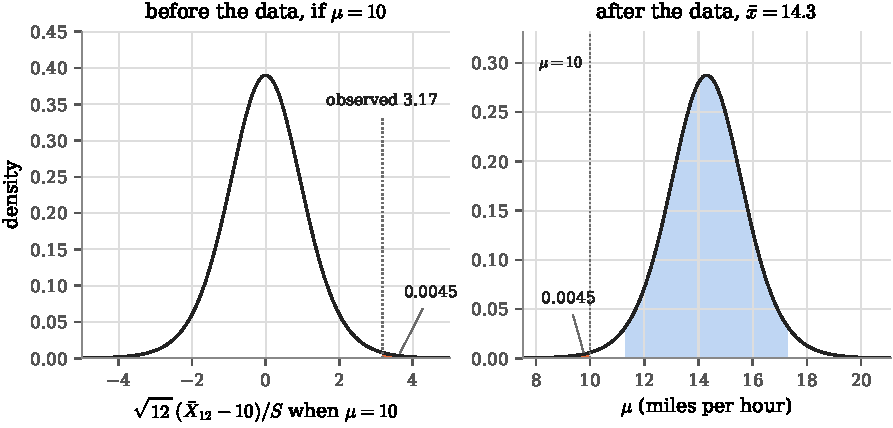
\includegraphics[width=\textwidth]{fig_jeffreys_t_two_readings}
\caption{One $t_{11}$ density read two ways, for the wind turbine. Left: the standardized mean when $\mu = 10$; orange, the area above the observed $3.17$. Right: the posterior of $\mu$ under the prior $1/\sigma$; orange, the area below $10$; blue, the $95\%$ $t$-interval.}
\label{fig:jefftreadings}
\end{figure}

\begin{bridge}[the $t$-interval is also a Bayesian interval]
An introductory course computes $\bar{x} \pm t^*s/\sqrt{n}$ and warns that `there is a $95\%$ probability that $\mu$ is in the interval' is the wrong sentence, since $\mu$ is fixed and the interval is random.
Under the prior flat in $\mu$ times $1/\sigma$, \cref{prop:jeff-t-posterior} makes that sentence true, with the same numbers: the probability is a posterior probability, conditional on the data, and it holds under this prior, not under every prior.
The $z$-interval with $\sigma$ known has the same double reading under the flat prior on $\mu$, whose posterior is $\Gauss(\bar{x}, \sigma^2/n)$.
\end{bridge}

\section{Bayesian confidence regions}
\label{sec:jeff-regions}

A posterior answers `where is $\theta$?' with a whole distribution.
A region that holds most of that distribution is the Bayesian counterpart of a confidence interval, and there is more than one way to choose it.

\begin{definition}[Bayesian confidence region]
\label{def:bayes-region}
Let $\alpha \in (0, 1)$, and let the posterior have a density. A \textbf{Bayesian confidence region of level $1 - \alpha$} is a set $R(\mathbf{x}) \subseteq \Theta$, computed from the data, with posterior probability $\Pr(\theta \in R(\mathbf{x}) \mid \mathbf{x}) = 1 - \alpha$. For a real parameter, the \textbf{equal-tailed} region is the interval from the point with posterior probability $\alpha/2$ below it to the point with posterior probability $\alpha/2$ above it. The \textbf{highest posterior density} region is $\{\theta : \pi(\theta \mid \mathbf{x}) \geq c\}$, with $c$ chosen so that its posterior probability is $1 - \alpha$.
\end{definition}

\begin{inwords}
\textbf{In words.} A region that holds $95\%$ of the posterior. The equal-tailed one cuts $2.5\%$ off each end; the highest-density one keeps the most probable values, those where the posterior density is above some height. Most texts call these credible regions, or credible intervals. This book calls $1 - \alpha$ the level, as for the confidence intervals of \cref{ch:confidence-intervals}, although some texts call $\alpha$ the level of a Bayesian region.
\par\smallskip
\textbf{For the kiss data.} Under Jeffreys' prior the posterior is $\Betad(80.5, 44.5)$. Its equal-tailed $95\%$ region is $[0.558, 0.725]$ and its highest-density region is $[0.560, 0.727]$, slightly to the right, toward the posterior's mode $0.646$: the posterior has a longer tail to the left.
\end{inwords}

The two kinds of region promise different things.
The highest-density region is the shortest region with the stated probability; the equal-tailed region follows the parameter through any monotone change of scale.

\begin{proposition}[The highest-density region is the shortest]
\label{prop:hpd-shortest}
Let the posterior have a density $f$ on $\real$, and let $H = \{\theta : f(\theta) \geq c\}$, with $c > 0$, have posterior probability $1 - \alpha$. Every set $R$ with posterior probability at least $1 - \alpha$ is at least as long as $H$.
\end{proposition}

\optionalproof{Compare the parts where $R$ and $H$ differ: the part only in $H$ has density at least $c$ and the part only in $R$ at most $c$, so $R$ needs at least as much length to hold at least as much probability.}
\begin{proof}
Write $\abs{A}$ for the length of a set $A$ and $P(A)$ for its posterior probability. Since $P(R) \geq P(H)$ and the two share $R \cap H$, $P(R \setminus H) \geq P(H \setminus R)$. On $R \setminus H$ the density is below $c$, so $P(R \setminus H) \leq c\abs{R \setminus H}$; on $H \setminus R$ it is at least $c$, so $P(H \setminus R) \geq c\abs{H \setminus R}$. Hence $c\abs{R \setminus H} \geq c\abs{H \setminus R}$, and dividing by $c$ and adding $\abs{R \cap H}$ to both sides gives $\abs{R} \geq \abs{H}$.
\end{proof}

The equal-tailed region has the other property.
If $\varphi = g(\theta)$ with $g$ increasing, the point with posterior probability $\alpha/2$ below it for $\varphi$ is $g$ of the corresponding point for $\theta$, so the equal-tailed region for $\varphi$ is the image of the one for $\theta$.
The highest-density region has no such guarantee, since the posterior density of $\varphi$ carries the factor $\abs{\mathrm{d}\theta/\mathrm{d}\varphi}$ of \cref{eq:jeff-change}, which changes which values count as most probable.

The wind turbine's $\sigma$ shows the difference.
Under the prior flat in $\mu$ times $1/\sigma$, integrating $\mu$ out of $\sigma^{-(n+1)}\exp(-A(\mu)/(2\sigma^2))$ leaves the posterior $\sigma^{-n}\exp(-(n-1)s^2/(2\sigma^2))$ for $\sigma$, since $A(\mu) = (n-1)s^2 + n(\mu - \bar{x})^2$ and the Gaussian integral $\int \exp(-n(\mu - \bar{x})^2/(2\sigma^2))\,\mathrm{d}\mu = \sigma\sqrt{2\pi/n}$ contributes one factor of $\sigma$.
The change of variables $v = (n-1)s^2/\sigma^2$, with $\sigma = s\sqrt{(n-1)/v}$ and $\abs{\mathrm{d}\sigma/\mathrm{d}v} \propto v^{-3/2}$, turns this into a density proportional to $v^{n/2}e^{-v/2}v^{-3/2} = v^{(n-1)/2 - 1}e^{-v/2}$, the $\chi^2_{n-1}$ density of \cref{prop:chisq-props}: $(n-1)s^2/\sigma^2$, with $\sigma$ random and $s$ fixed, has the $\chi^2_{n-1}$ distribution.
That is the distribution Cochran's theorem (\cref{thm:cochran}) gives $(n-1)S^2/\sigma^2$ over repeated samples, so here too the equal-tailed region coincides with the frequentist interval built from that pivot: $[3.33, 7.98]$ for $\sigma$ and, squared, $[11.1, 63.7]$ for $\sigma^2$.
The highest-density regions are $[3.08, 7.45]$ for $\sigma$ and $[8.5, 53.9]$ for $\sigma^2$, each shorter than the equal-tailed region on its own scale.
But the square of the first is $[9.5, 55.5]$, not the second: shortest on the scale of $\sigma$ and shortest on the scale of $\sigma^2$ are different requirements.
\Cref{fig:jeffhpd} shows both scales.

\begin{figure}[htbp]
\centering
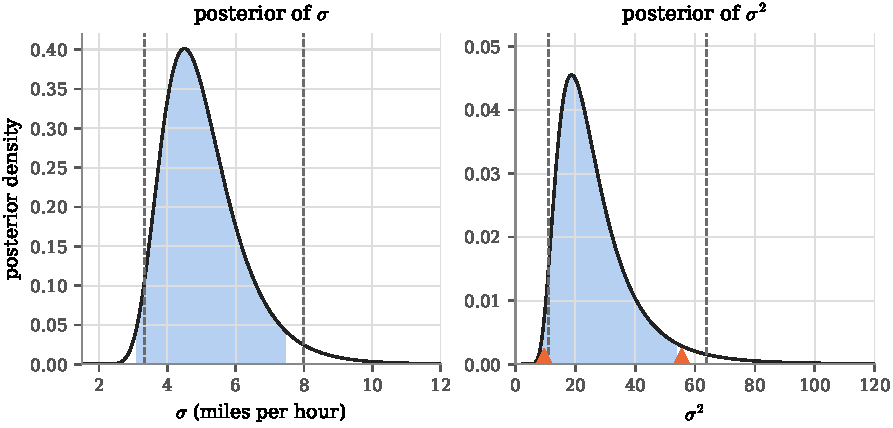
\includegraphics[width=\textwidth]{fig_jeffreys_hpd}
\caption{Posterior of the wind turbine's $\sigma$ (left) and $\sigma^2$ (right) under the prior $1/\sigma$. Blue: the $95\%$ highest-density regions. Gray dashed: the equal-tailed regions. Orange triangles: the squares of the endpoints of the left highest-density region.}
\label{fig:jeffhpd}
\end{figure}

\begin{pitfall}[the shortest region depends on the scale]
`The $95\%$ highest-density interval' is not a property of the posterior alone: it also depends on whether length is measured in $\sigma$ or in $\sigma^2$, in $p$ or in $\psi$.
When the parameterization is a matter of convention, report the equal-tailed region, which follows the parameter through every monotone change of scale, or say on which scale the highest-density region was computed.
\end{pitfall}

The subway shows the same exact coincidence for a rate.
Under Jeffreys' prior its posterior is $\Gammad(64, 398.7)$, whose $2.5\%$ and $97.5\%$ points are $49.29/398.7 = 0.124$ and $80.60/398.7 = 0.202$, where $49.29$ and $80.60$ are the corresponding points of $\Gammad(64, 1)$.
That is exactly the interval of \cref{ex:ci-gamma}, built from the pivot $\lambda\sum_i T_i \sim \Gammad(64, 1)$.
Again one distribution is read twice: over repeated samples with $\lambda$ fixed, $\lambda\sum_i T_i$ is $\Gammad(64, 1)$; over $\lambda$ with the sample fixed, the posterior $\Gammad(64, 398.7)$ makes $398.7\lambda$ a $\Gammad(64, 1)$ variable.
The two sentences come apart only in what they are about.
`Of $1{,}000$ subway studies of $64$ waits each, the interval computed from each covers the true rate in about $950$' is a statement about the procedure.
`Given these $64$ waits and Jeffreys' prior, the rate lies in $[0.124, 0.202]$ with probability $0.95$' is a statement about $\lambda$: the first of the three readings that \cref{sec:ci-meaning} ruled out for a confidence interval, true here under a prior.

\begin{sanitycheck}[Should the posterior mean wait be $1/0.1605$?]
Under Jeffreys' prior the posterior mean of the rate is $64/398.7 = 0.1605$, the maximum likelihood estimate, so it is tempting to call $1/0.1605 = 6.23$ minutes the posterior mean of the wait.
It is not: the wait $\beta = 1/\lambda$ has posterior mean $\E[1/\lambda \mid \text{data}] = 398.7/63 = 6.33$ minutes, larger, as Jensen's inequality says it must be, since $1/\lambda$ is convex \toolkit{sec:math-convex}.
Means do not follow a nonlinear change of scale, but quantiles do: the posterior median of the rate is $0.1597$, and the posterior median of the wait is $1/0.1597 = 6.26$ minutes.
\end{sanitycheck}

\section{When the two kinds of interval agree}
\label{sec:jeff-agree}

The exact coincidences of the last two sections, the $z$- and $t$-intervals, the chi-squared interval for $\sigma$ and the subway's Gamma interval, all come from location and scale families with the matching improper prior, flat for a location and $1/\text{scale}$ for a scale: there the posterior distribution of the pivot equals its sampling distribution.
In other models the two kinds of interval agree only approximately, and the Bernstein--von Mises theorem says how.

\recall{The Bernstein--von Mises theorem (\cref{thm:bvm}): for i.i.d.\ data from a model satisfying the regularity conditions of \cref{sec:mle-regularity}, with $\theta^*$ in the interior of $\Theta$, $I(\theta^*) > 0$, data that separate $\theta^*$ from distant values, and a prior density continuous and positive at $\theta^*$, the posterior distribution of $\sqrt{n}(\theta - \hat{\theta}_n)$ approaches $\Gauss(0, 1/I(\theta^*))$ in total variation, in probability. Slutsky's theorem (\cref{thm:slutsky}): if $X_n \convd X$ and $Y_n \convp c$ for a constant $c$, then $X_n + Y_n \convd X + c$.}

Closeness in total variation makes every posterior probability, and so every posterior quantile of $\sqrt{n}(\theta - \hat{\theta}_n)$, close to the Gaussian one.
So the equal-tailed region of level $1 - \alpha$ is $\hat{\theta}_n \pm q_{\alpha/2}/\sqrt{nI(\theta^*)}$ up to an error that is negligible next to $1/\sqrt{n}$.
It covers $\theta^*$ exactly when $\sqrt{n}(\hat{\theta}_n - \theta^*)$ lies between $-q_{\alpha/2}/\sqrt{I(\theta^*)}$ and $q_{\alpha/2}/\sqrt{I(\theta^*)}$, each moved by a term that converges to $0$ in probability, so by \cref{thm:mle-normal} and Slutsky's theorem, applied at each end, the Bayesian region has asymptotic coverage $1 - \alpha$, the same as the plug-in interval $\hat{\theta}_n \pm q_{\alpha/2}/\sqrt{nI(\hat{\theta}_n)}$ of \cref{ch:mle-properties}, whatever the prior, as long as its density is continuous and positive at $\theta^*$.
With an improper prior the same can be checked in each example of this chapter, whose posteriors are explicit.
For the kiss data the priors of this chapter give $95\%$ regions within $0.003$ of each other and of the solve interval of \cref{ch:confidence-intervals}, $[0.558, 0.724]$: flat $[0.558, 0.724]$, Jeffreys $[0.558, 0.725]$, Haldane $[0.559, 0.727]$.

How fast the agreement comes depends on the prior, and for one-sided bounds Jeffreys' prior is special.
For a one-parameter model with continuous data, Welch and Peers (\textit{Journal of the Royal Statistical Society B}, 1963) showed that the posterior's one-sided bounds have frequentist coverage $1 - \alpha$ up to an error of order $1/n$ when the prior is Jeffreys', and of order only $1/\sqrt{n}$ for other smooth priors.
In an equal-tailed region the two errors of order $1/\sqrt{n}$ cancel, so its coverage error is of order $1/n$ under any smooth prior.
These results are stated without proof; their proof needs more than this book develops, and nothing later depends on them.
For a proportion no interval has coverage exactly $1 - \alpha$ at every $p$, since the data are discrete, but the Jeffreys interval, the equal-tailed region of $\Betad(S + \frac12, n - S + \frac12)$, comes close.
At $p = 0.645$ and $n = 124$ its coverage is $0.952$, the same as the solve interval's, where the plug-in interval has $0.939$.
At $n = 20$, averaged over $p$ from $0.01$ to $0.99$, the coverage is $0.951$ for the Jeffreys interval, $0.954$ for the solve interval and $0.861$ for the plug-in interval.
\Cref{fig:jeffcoverage} draws the solve and Jeffreys intervals at $n = 20$: both oscillate around $0.95$, the solve interval dropping lowest at the very ends ($0.84$ just below $p = 0.009$) and the Jeffreys interval at $p = 0.12$ and $0.88$ ($0.89$).
Of $1{,}000$ studies of $20$ couples, the Jeffreys interval covers the true $p$ in about $951$ on average over $p$, the plug-in interval in about $861$.
Brown, Cai and DasGupta (\textit{Statistical Science}, 2001) recommend the solve (Wilson) interval or the Jeffreys interval for small $n$, the latter modified when $S$ is $0$, $1$, $n - 1$ or $n$: as defined here, the interval for $S = 0$ starts above $0$ (at $0.000024$ when $n = 20$), so its coverage is $0$ for $p$ closer to $0$ than that.

\begin{figure}[htbp]
\centering
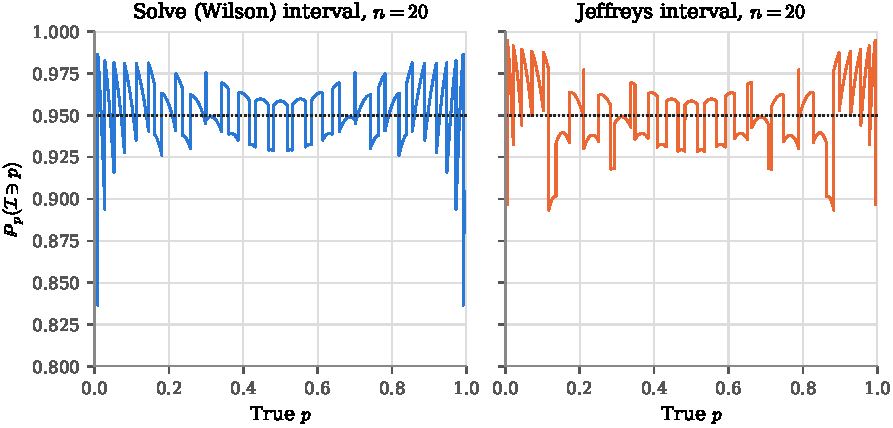
\includegraphics[width=\textwidth]{fig_jeffreys_coverage}
\caption{Exact coverage $\Pr_p(\mathcal{I} \ni p)$ of two $95\%$ intervals for a proportion at $n = 20$, against the true $p$: left, the solve (Wilson) interval (blue); right, the equal-tailed Jeffreys interval (orange). Dotted: the nominal $0.95$.}
\label{fig:jeffcoverage}
\end{figure}

The agreement has limits, and \cref{ch:bayes-intro} has already shown two.
With an informative prior and moderate $n$ the regions differ: the skeptic's prior gave the interval $[0.56, 0.73]$ posterior probability $0.835$, not $0.95$.
For a point null the answers differ at every $n$: a prior with a lump of probability at $p = \frac12$ has no density, so the Bernstein--von Mises theorem does not apply, and $\Pr(H_0 \mid \mathbf{x}) = 0.044$ stood against a $p$-value of $0.0012$.

\section{What comes next}
\label{sec:jeff-next}

This chapter ends Part VII.
Part VIII returns to the frequentist methods of the earlier parts and applies them to a model with a predictor, the linear regression model of \cref{ch:regression-uni}, where least squares, the method that led Gauss to the distribution named after him (\cref{ch:gaussian}), is the estimator.
The Bayesian reading carries over: with Gaussian errors, the least squares estimate is the posterior mode under a flat prior on the coefficients, and with a Gaussian prior centered at zero the posterior mode is the ridge estimate that \cref{ch:bayes-intro} mentioned.

\section{Summary}
\label{sec:jeff-summary}

\begin{itemize}[nosep]
\item A flat prior is flat on one scale only. By the change of variables formula $\pi_\varphi = \pi_\theta\abs{\mathrm{d}\theta/\mathrm{d}\varphi}$, flat in $p$ is the logistic density in the log-odds, and flat in the subway's mean wait is $1/\lambda^2$ in terms of the rate; at $n = 64$ the two flat answers for the subway differ by a quarter of a posterior standard deviation.
\item An improper prior has an infinite integral. It gives a posterior when $0 < \int L_n\pi < \infty$, and none otherwise (Haldane's prior when every couple turns right). It can be read as the limit of wider and wider proper priors, and its arbitrary constant cancels in estimation but makes the Bayes factor arbitrary when it is the prior for the parameter that a point null fixes.
\item Fisher information changes with the parameterization as $I_\varphi = I_\theta(\mathrm{d}\theta/\mathrm{d}\varphi)^2$, so Jeffreys' prior $\pi_J \propto \sqrt{I}$, or $\sqrt{\det I}$ in several dimensions, is the same prior whichever parameterization it is computed in. It gives equal mass to intervals the data can just tell apart, and it is flat on the variance-stabilizing scale $\int\sqrt{I}$: $2\arcsin\sqrt{p}$, $2\sqrt{\lambda}$, $\log\lambda$.
\item Jeffreys' priors: $\Betad(\frac12, \frac12)$ for a proportion (kiss posterior mean $0.644$), $\lambda^{-1/2}$ for a Poisson mean, $1/\lambda$ for a rate (subway posterior mean $0.1605$, the maximum likelihood estimate), flat for a Gaussian mean, $1/\sigma$ for a scale. For a Gaussian with both parameters unknown the joint rule gives $1/\sigma^2$, and the product of the separate rules, $1/\sigma$, is the one that reproduces the $t$-interval.
\item A Bayesian confidence region of level $1 - \alpha$ has posterior probability $1 - \alpha$. The highest-density region is the shortest; the equal-tailed region follows the parameter through any monotone change of scale, and the highest-density region does not.
\item With the matching improper prior, Bayesian regions equal frequentist intervals exactly in location and scale families: the $z$- and $t$-intervals, the chi-squared interval for $\sigma$, the subway's exact $[0.124, 0.202]$. Elsewhere they agree as $n$ grows (Bernstein--von Mises); for one-sided bounds the agreement is fastest under Jeffreys' prior (Welch and Peers), and the Jeffreys interval for a proportion covers about $95\%$ of the time on average over $p$ even at $n = 20$.
\end{itemize}

\section{Exercises}
\label{sec:jeff-exercises}

\begin{exercise}
\label{ex:jeff-poisson}
(a) Show that Jeffreys' prior for the Poisson mean is $\lambda^{-1/2}$, that it is improper, and that after $n \geq 1$ observations with sum $S$ the posterior is $\Gammad(S + \frac12, n)$. (b) The siblings data of \cref{ch:models} have $24$ values of $X - 1$ adding up to $24$. Find the posterior mean of $\lambda$ under Jeffreys' prior and under the flat prior $\pi(\lambda) = 1$, and compare with the maximum likelihood estimate.
\end{exercise}
\begin{solution}
(a) $I(\lambda) = 1/\lambda$ (\cref{sec:mle-fisher-examples}), so $\pi_J(\lambda) \propto \lambda^{-1/2}$, and $\int_0^M \lambda^{-1/2}\,\mathrm{d}\lambda = 2\sqrt{M} \to \infty$: improper. The likelihood is proportional to $\lambda^{S}e^{-n\lambda}$, so the posterior is proportional to $\lambda^{S - 1/2}e^{-n\lambda}$, the $\Gammad(S + \frac12, n)$ density, whose integral is finite for every $S \geq 0$ once $n \geq 1$. (b) Jeffreys: $\Gammad(24.5, 24)$, mean $24.5/24 = 1.021$. Flat: $\Gammad(25, 24)$, mean $25/24 = 1.042$. The maximum likelihood estimate is $24/24 = 1$. Jeffreys' prior adds half a count to $S$ and the flat prior a whole count.
\end{solution}

\begin{exercise}
\label{ex:jeff-geometric}
A geometric observation counts the trials up to and including the first success, $\Pr_p(X = x) = p(1-p)^{x-1}$ for $x = 1, 2, \ldots$, with $\E_p[X] = 1/p$. (a) Show that $I(p) = 1/(p^2(1-p))$, so Jeffreys' prior is $p^{-1}(1-p)^{-1/2}$, and that it is improper. (b) Suppose an observer watched kissing couples until the first right turn, five times over, needing $1$, $2$, $1$, $1$ and $3$ couples. Show that Jeffreys' posterior is $\Betad(5, 3.5)$ and find its mean. (c) The same eight couples, read as eight Bernoulli trials with five right turns, have a likelihood proportional to the same function of $p$. What is Jeffreys' posterior mean for them, and what does the difference say about Jeffreys' prior?
\end{exercise}
\begin{solution}
(a) $\ell(p) = \log p + (X - 1)\log(1-p)$, so $\ell''(p) = -1/p^2 - (X - 1)/(1-p)^2$, and with $\E_p[X - 1] = (1-p)/p$, $I(p) = 1/p^2 + 1/(p(1-p)) = (1 - p + p)/(p^2(1-p)) = 1/(p^2(1-p))$. So $\pi_J(p) \propto p^{-1}(1-p)^{-1/2}$, whose integral diverges at $p = 0$ like $\int \mathrm{d}p/p$. (b) The likelihood of $n = 5$ observations with sum $8$ is $p^5(1-p)^{8-5}$, and times the prior it is $p^4(1-p)^{2.5}$: the $\Betad(5, 3.5)$ density, with mean $5/8.5 = 0.588$. (c) Jeffreys' prior for Bernoulli trials is $\Betad(\frac12, \frac12)$, and the posterior is $\Betad(5.5, 3.5)$, with mean $5.5/9 = 0.611$. The likelihoods are the same, but the priors differ because the Fisher information depends on how the data were collected, not only on the likelihood they produced: Jeffreys' prior depends on the sampling plan.
\end{solution}

\begin{exercise}
\label{ex:jeff-scale}
Let $\Xton \iid \Gauss(\mu, v)$ with $\mu$ known, parameterized by the variance $v = \sigma^2$. (a) Show that Jeffreys' prior for $v$ is proportional to $1/v$. (b) Show that carrying the prior $1/\sigma$ on $\sigma$ to $v$ by \cref{eq:jeff-change} gives $1/v$ up to a constant, as \cref{thm:jeffreys-invariant} says it must. (c) Show that the prior $1/\sigma$ is the flat prior on $\log\sigma$, and that rescaling, $\sigma' = c\sigma$ for a constant $c > 0$, such as a change from miles to kilometers per hour, leaves it in the same form.
\end{exercise}
\begin{solution}
(a) By \cref{sec:mle-fisher-examples}, the information for the variance is $1/(2v^2)$, and its square root is $1/(\sqrt{2}\,v) \propto 1/v$. (b) $\sigma = \sqrt{v}$ and $\mathrm{d}\sigma/\mathrm{d}v = 1/(2\sqrt{v})$, so the prior on $v$ is $\frac{1}{\sqrt{v}} \cdot \frac{1}{2\sqrt{v}} = \frac{1}{2v} \propto \frac1v$. (c) With $\eta = \log\sigma$, $\mathrm{d}\eta/\mathrm{d}\sigma = 1/\sigma$, so a constant density in $\eta$ is $1/\sigma$ in $\sigma$ by \cref{eq:jeff-change}. Under $\sigma' = c\sigma$, $\mathrm{d}\sigma/\mathrm{d}\sigma' = 1/c$ and $\pi(\sigma') = \frac{1}{\sigma'/c} \cdot \frac1c = \frac{1}{\sigma'}$, the same form.
\end{solution}

\begin{exercise}
\label{ex:jeff-haldane}
(a) Show that under Haldane's prior $\pi(p) = 1/(p(1-p))$ the posterior after $S$ successes in $n$ trials is $\Betad(S, n - S)$ when $0 < S < n$, and that its mean is the sample proportion. (b) Show that there is no posterior when $S = 0$, and that under Jeffreys' prior there is one for every $S$. (c) Give the posterior means of $p$ for the kiss data under the flat, Jeffreys and Haldane priors, and say which way each prior pulls the estimate.
\end{exercise}
\begin{solution}
(a) $L_n\pi = p^S(1-p)^{n-S}/(p(1-p)) = p^{S-1}(1-p)^{n-S-1}$, integrable when $S \geq 1$ and $n - S \geq 1$; it is the $\Betad(S, n - S)$ density, with mean $S/n$. (b) With $S = 0$, $L_n\pi = p^{-1}(1-p)^{n-1}$, whose integral diverges at $p = 0$ like $\int \mathrm{d}p/p$, so $m(\mathbf{x}) = \infty$. Under Jeffreys' prior the posterior is $\Betad(S + \frac12, n - S + \frac12)$, both of whose parameters are at least $\frac12$ for every $S$. (c) Flat: $81/126 = 0.643$; Jeffreys: $80.5/125 = 0.644$; Haldane: $80/124 = 0.645$. The flat prior adds one imaginary success and one failure and pulls toward $\frac12$ the most, Jeffreys' prior adds half of each, and Haldane's adds none.
\end{solution}

\begin{exercise}
\label{ex:jeff-subway-wait}
For the subway, under each of the three priors of this chapter for the rate (flat in $\lambda$, Jeffreys' $1/\lambda$, flat in the wait $\beta$), the posterior of $\lambda$ is $\Gammad(a, 398.7)$ with $a = 65$, $64$ and $63$. (a) Show that the posterior mean of the wait $\beta = 1/\lambda$ is $398.7/(a - 1)$, and compute it for the three priors. (b) The $95\%$ equal-tailed regions for $\lambda$ are $[0.1258, 0.2050]$, $[0.1236, 0.2022]$ and $[0.1214, 0.1994]$. Give the equal-tailed regions for $\beta$ without further computation. (c) Which prior makes the posterior mean of $\beta$ equal to the maximum likelihood estimate $6.23$, and which makes the posterior mean of $\lambda$ equal to $1/6.23$?
\end{exercise}
\begin{solution}
(a) $\E[1/\lambda] = \int_0^\infty \frac1\lambda\,\frac{b^a}{\Gamma(a)}\lambda^{a-1}e^{-b\lambda}\,\mathrm{d}\lambda = \frac{b^a}{\Gamma(a)}\cdot\frac{\Gamma(a-1)}{b^{a-1}} = \frac{b}{a-1}$, using $\Gamma(a) = (a-1)\Gamma(a-1)$. With $b = 398.7$: $6.23$, $6.33$ and $6.43$ minutes. (b) The map $\lambda \mapsto 1/\lambda$ is decreasing, so the equal-tailed region for $\beta$ is $[1/U, 1/L]$: $[4.88, 7.95]$, $[4.95, 8.09]$ and $[5.02, 8.24]$ minutes. (c) The flat prior on $\lambda$ ($a = 65$) gives posterior mean wait $398.7/64 = 6.23$; Jeffreys' prior ($a = 64$) gives posterior mean rate $64/398.7 = 0.1605 = 1/6.23$. No prior makes both means equal to the maximum likelihood estimates, since $\E[1/\lambda] > 1/\E[\lambda]$.
\end{solution}

\begin{exercise}
\label{ex:jeff-joint}
Under the prior $1/\sigma^2$ of \cref{prop:jeff-t-posterior}, the $95\%$ equal-tailed region for $\mu$ is $\bar{x} \pm q_{0.025}(t_n)\sqrt{(n-1)/n}\,s/\sqrt{n}$. (a) Show that, read as a confidence interval, its coverage is $\Pr(\abs{T} \leq q_{0.025}(t_n)\sqrt{(n-1)/n})$ with $T \sim t_{n-1}$, whatever $\mu$ and $\sigma$ are. (b) Evaluate it at $n = 5$, given $q_{0.025}(t_5) = 2.5706$ and $\Pr(\abs{t_4} \leq 2.299) = 0.917$. (c) What is the coverage of the region under the prior $1/\sigma$?
\end{exercise}
\begin{solution}
(a) The interval contains $\mu$ exactly when $\abs{\sqrt{n}(\bar{X}_n - \mu)/S} \leq q_{0.025}(t_n)\sqrt{(n-1)/n}$, and by \cref{thm:t-pivot} the left side is $\abs{T}$ with $T \sim t_{n-1}$ for every $\mu$ and $\sigma$. (b) $2.5706 \times \sqrt{4/5} = 2.299$, so the coverage is $0.917$, against the nominal $0.95$; at $n = 12$ it is $0.939$. (c) Exactly $0.95$: under $1/\sigma$ the region is $\bar{x} \pm q_{0.025}(t_{n-1})s/\sqrt{n}$, the $t$-interval.
\end{solution}

\begin{exercise}
\label{ex:jeff-bayes-factor}
Test $H_0: p = \frac12$ against $H_1: p \neq \frac12$ for the kiss data, with prior probability $\frac12$ on each, as in \cref{sec:bayes-hypotheses}, but with Haldane's prior $c/(p(1-p))$ on $H_1$. (a) Show that $m_1 = c\,B(80, 44)$, where $B(a, b) = \int_0^1 p^{a-1}(1-p)^{b-1}\,\mathrm{d}p$. (b) Given $B(80, 44) = 4.45 \times 10^{-36}$ and $m_0 = 2^{-124} = 4.70 \times 10^{-38}$, compute $B_{01}$ and $\Pr(H_0 \mid \mathbf{x})$ for $c = 1$ and for $c = 1{,}000$. (c) Why does the constant not matter when the same prior is used to estimate $p$?
\end{exercise}
\begin{solution}
(a) $m_1 = \int_0^1 p^{80}(1-p)^{44}\,\frac{c}{p(1-p)}\,\mathrm{d}p = c\int_0^1 p^{79}(1-p)^{43}\,\mathrm{d}p = c\,B(80, 44)$. (b) $c = 1$: $B_{01} = 4.70 \times 10^{-38}/(4.45 \times 10^{-36}) = 0.0106$ and $\Pr(H_0 \mid \mathbf{x}) = 0.0106/1.0106 = 0.0105$. $c = 1{,}000$: $B_{01} = 1.06 \times 10^{-5}$ and $\Pr(H_0 \mid \mathbf{x}) = 1.06 \times 10^{-5}$. Nothing in the data or the model picks $c$. (c) The posterior under $H_1$ is $c\,p^{79}(1-p)^{43}/(c\,B(80, 44))$, and $c$ cancels.
\end{solution}

\begin{exercise}
\label{ex:jeff-symmetric}
(a) Show that if a posterior density on $\real$ is symmetric about a point $m$ and decreases as $\abs{\theta - m}$ grows, its highest-density and equal-tailed regions of every level coincide. (b) Which posteriors of this chapter are of that kind, and which are not?
\end{exercise}
\begin{solution}
(a) The set where the density is at least $c$ is an interval $[m - h, m + h]$, symmetric about $m$, and by symmetry it leaves the same posterior probability $\alpha/2$ outside it on each side. So the highest-density region with probability $1 - \alpha$ is the equal-tailed one. (b) The posterior $\Gauss(\bar{x}, \sigma^2/n)$ of a Gaussian mean and the $t$ posteriors of \cref{prop:jeff-t-posterior} are of that kind. The Beta posteriors of the kiss data, the Gamma posteriors of the subway and the posteriors of $\sigma$ and $\sigma^2$ are skewed, and there the two regions differ.
\end{solution}

\begin{exercise}
\label{ex:jeff-location}
Let $X$ have density $f(x - \theta)$, with $f$ a known density on $\real$ (a location family), and take the improper prior $\pi(\theta) = 1$. (a) Show that the posterior density of $\theta$ given $X = x$ is $f(x - \theta)$. (b) Let $u(x)$ be the posterior's upper bound of level $1 - \alpha$: $\Pr(\theta \leq u(x) \mid x) = 1 - \alpha$. Show that $\Pr_\theta(\theta \leq u(X)) = 1 - \alpha$ for every $\theta$: the Bayesian bound has exact frequentist coverage.
\end{exercise}
\begin{solution}
(a) $L(x; \theta)\pi(\theta) = f(x - \theta)$, and $\int f(x - \theta)\,\mathrm{d}\theta = \int f(w)\,\mathrm{d}w = 1$, so $m(x) = 1$ and the posterior is $f(x - \theta)$. (b) Given $x$, $\theta = x - W$ with $W$ having density $f$, so $\theta \leq u(x)$ exactly when $W \geq x - u(x)$. The posterior condition says $\Pr(W \geq x - u(x)) = 1 - \alpha$, so $x - u(x) = w$, the point with probability $\alpha$ below it under $f$, the same for every $x$, and $u(x) = x - w$. Under $\Pr_\theta$, $X = \theta + W'$ with $W'$ having density $f$, and $\theta \leq X - w$ exactly when $W' \geq w$, which has probability $1 - \alpha$.
\end{solution}

\begin{exercise}
\label{ex:jeff-drug}
In the drug trial of \cref{ch:kiss}, $78$ of $100$ patients were cured. (a) Give Jeffreys' posterior, its mean and its $95\%$ equal-tailed region, given that the $2.5\%$ and $97.5\%$ points of the posterior are $0.692$ and $0.852$. (b) Compute the arcsine interval $2\arcsin\sqrt{\hat{p}} \pm 1.96/\sqrt{n}$, mapped back to $p$, and compare with (a), with the solve interval $[0.689, 0.850]$ of \cref{eq:wilson} and with the plug-in interval $[0.699, 0.861]$ of \cref{ch:kiss}.
\end{exercise}
\begin{solution}
(a) $\Betad(78.5, 22.5)$, with mean $78.5/101 = 0.777$ and $95\%$ region $[0.692, 0.852]$. (b) $2\arcsin\sqrt{0.78} = 2.165$ and $1.96/\sqrt{100} = 0.196$, so $\varphi \in [1.969, 2.361]$, and $p = \sin^2(\varphi/2)$ gives $[0.694, 0.855]$. The Jeffreys, arcsine and solve intervals agree to within about $0.005$ and all sit to the left of the plug-in interval, which is symmetric about $0.78$ although the binomial is skewed this close to $1$.
\end{solution}
